\documentclass[10pt,journal,twocolumn]{IEEEtran} % add 'draft' to suppress figures
% Double-spaced, single-column format for IEEE journal submission
% \documentclass[12pt,journal,draftclsnofoot,onecolumn]{IEEEtran} 
\usepackage{wrapfig,booktabs,fancyhdr,amsmath,amsfonts,tabularx,numprint}
\usepackage{cite,bm,bbm,amssymb,amsthm,url,multirow,times,enumitem,comment}
\usepackage{mathtools,siunitx,balance,tikz,adjustbox,graphicx,array}
\usepackage[font=footnotesize]{subcaption}
\usepackage[linesnumbered,ruled]{algorithm2e}
\usepackage[colorlinks=true, linkcolor=black, citecolor=blue, urlcolor=blue]{hyperref}
\newcommand{\vb}{\boldsymbol}
\newcommand{\vbh}[1]{\hat{\boldsymbol{#1}}}
\newcommand{\vbc}[1]{\check{\boldsymbol{#1}}}
\newcommand{\vbb}[1]{\bar{\boldsymbol{#1}}}
\newcommand{\vbt}[1]{\tilde{\boldsymbol{#1}}}
\newcommand{\vbs}[1]{{\boldsymbol{#1}}^*}
\newcommand{\vbd}[1]{\dot{{\boldsymbol{#1}}}}
\newcommand{\abs}[1]{\left|{#1}\right|}
\newcommand{\by}{\times}
\newcommand{\tr}{\mathsf{T}}
\newcommand{\sfrac}[2]{\textstyle \frac{#1}{#2}}
\newcommand{\ba}{\begin{array}}
\newcommand{\ea}{\end{array}}
\newcommand{\sinc}{\text{sinc}}
\newcommand{\define}{\triangleq}
%\newcommand{\define}{\coloneqq}
\newcommand{\cnr}{C/N_0}
\newcommand{\sgn}{\text{sgn}}
\renewcommand{\Re}{\mathbb{R}}
\renewcommand{\Im}{\mathbb{I}}
\newcommand{\E}[1]{\mathbb{E}\left[ #1 \right]}
\newcommand{\brm}[1]{\bm{\text{#1}}}
\newcommand{\round}[1]{\ensuremath{\lfloor#1\rceil}}
\DeclareMathAlphabet{\mathpzc}{OT1}{pzc}{m}{it}
\DeclareMathOperator*{\argmin}{\arg\!\min}
\DeclareMathOperator*{\argmax}{\arg\!\max}

% Macros for this paper
\newcommand{\Fc}[1]{\ensuremath{F_{\text{c}#1}}}
\newcommand{\Fs}{\ensuremath{F_\text{s}}}
\newcommand{\Fsr}{\ensuremath{F_\text{sr}}}

% \topmargin = 0 mm 
% \oddsidemargin = -1 mm 
% \evensidemargin = -1 mm
% \headheight = 0 mm 
% \headsep = 8 mm 
% \textheight = 220 mm 
% \textwidth =170 mm 
% \parindent = 0 mm
% \parskip = 4 mm 

\begin{document}
%%% ----------------------------------------------------------Front Matter
\title{An Exegesis of Ontological Hermeneutics}

\author{
  \IEEEauthorblockN{Gandalf the White\IEEEauthorrefmark{1}, Radagast the
    Brown\IEEEauthorrefmark{2}, Todd E. Humphreys\IEEEauthorrefmark{1}} \\
  \IEEEauthorblockA{\IEEEauthorrefmark{1}\textit{Department of Aerospace
      Engineering and Engineering Mechanics, The University of Texas at Austin}} \\
  \IEEEauthorblockA{\IEEEauthorrefmark{2}\textit{Department of Elven Lore, The
    University of East Rivendell}}
}

\maketitle

\begin{abstract}
  The abstract is a one-paragraph summary of the whole paper.  Out of respect
  for busy readers, it gets right to the point.  The first 2-3 sentences
  unpack the title and motivate the paper.  The remainder briefly offers
  context (if necessary) and further describes the paper's method, explaining
  how it fills a gap in the existing literature.  The abstract reveals all the
  paper's main results in language that is bold but truthful.

An example for a paper titled ``Deep urban unaided precise GNSS vehicle
positioning'': \\ \\ 

This paper presents the most thorough study to date of vehicular carrier-phase
differential GNSS (CDGNSS) positioning performance in a deep urban setting
unaided by complementary sensors.  Using data captured during approximately 2
hours of driving in and around the dense urban center of Austin, TX, a CDGNSS
system is demonstrated to achieve 17-cm-accurate 3D urban positioning (95\%
probability) with solution availability greater than 87\%.  The results are
achieved without any aiding by inertial, electro-optical, or odometry sensors.
Development and evaluation of the unaided GNSS-based precise positioning
system is a key milestone toward the overall goal of combining precise GNSS,
vision, radar, and inertial sensing for all-weather high-integrity
high-absolute-accuracy positioning for automated and connected vehicles.  The
system described and evaluated herein is composed of a densely-spaced
reference network, a software-defined GNSS receiver, and a real-time kinematic
(RTK) positioning engine.  A performance sensitivity analysis reveals that
navigation data wipeoff for fully-modulated GNSS signals and a dense reference
network are key to high-performance urban RTK positioning.  A comparison with
existing unaided systems for urban GNSS processing indicates that the proposed
system has significantly greater availability or accuracy.
\end{abstract}

\begin{IEEEkeywords} 
urban vehicular positioning; CDGNSS; low-cost RTK positioning.
\end{IEEEkeywords}

%%% -------------------------- Select preprint or "for submission" version
\newif\ifpreprint
\preprintfalse
%\preprinttrue

\ifpreprint

\pagestyle{plain}
\thispagestyle{fancy}  
\fancyhf{} 
\renewcommand{\headrulewidth}{0pt}
\rfoot{\footnotesize \bf October 2020 preprint of paper submitted for review} \lfoot{\footnotesize \bf
  Copyright \copyright~2020 by Lakhsay Narula \\ and Todd E. Humphreys}

\else

\thispagestyle{empty}
\pagestyle{empty}

\fi

%%% ----------------------------------------------------------------------

\section{Introduction}
In the introduction:
\begin{itemize}
\item {\bf Background:} Set the stage in a compelling way to draw the reader
  in.
\item {\bf Opportunity/Need:} Identify a need or an opportunity.
\item {\bf The status quo:} Review the state of the art.  
\item {\bf Gap:} Mind the gap!  Convince your reader that there is an
  important deficiency (gap) in the existing literature or practice, and that
  your paper will save the day by filling in/bridging this gap.  Otherwise,
  why should your reader take time to read the paper?
\item {\bf Vision:} Invite the reader to imagine the way the world could be if
  only the gap could be bridged.
\item {\bf Contributions:} Clearly enumerate the paper's contributions.
\end{itemize}

What follows is an example introduction taken from
\cite{humphreys2019deepUrbanIts}. \\ \\ 

\IEEEPARstart{F}{uture} Vehicle-to-vehicle (V2V) and vehicle-to-infrastructure
(V2I) connectivity will permit vehicles to relay their positions and
velocities to each other with millisecond latency, enabling tight coordinated
platooning and efficient intersection management.  More ambitiously, broadband
V2V and V2I enabled by 5G wireless networks will permit vehicles to share
unprocessed or lightly-processed sensor data. \emph{Ad hoc} networks of
vehicles and infrastructure will then function as a single sensing organism.
The risk of collisions, especially with pedestrians and cyclists---notoriously
unpredictable and much harder to sense reliably than vehicles---will be
significantly reduced as vehicles and infrastructure contribute sensor data
from multiple vantage points to build a blind-spot-free model of their
surroundings.

Such collaborative sensing and traffic coordination requires vehicles to know
and share their own position.  How accurately?  The proposed Dedicated Short
Range Communications (DSRC) basic safety message, a first step in V2V
coordination, does not yet define a position accuracy requirement, effectively
accepting whatever accuracy a standard GNSS receiver provides
\cite{kenney2011dedicated}.  But automated intersection management
\cite{fajardo2011automated}, tight-formation platooning, and unified
processing of sensor data---all involving vehicles of different makes that may
not share a common map---will be greatly facilitated by globally-referenced
positioning with sub-30-cm accuracy.

Poor weather also motivates high-accuracy absolute positioning.  Every
automated vehicle initiative of which the present authors are aware depends
crucially on lidar or cameras for fine-grained positioning within their local
environment.  But these sensing modalities perform poorly in low-visibility
conditions such as a snowy whiteout, dense fog, or heavy rain.  Moreover,
high-definition 3D maps created with lidar and camera data, maps that have
proven crucial to recent progress in reliable vehicle automation, can be
rendered dangerously obsolete by a single snowstorm, leaving vehicles who rely
on such maps for positioning no option but to fall back on GNSS and radar to
navigate a snow-covered roadway in low-visibility conditions.  When, as is
often the case on rural roads, such snowy surroundings offer few
radar-reflective landmarks, radar too becomes useless.  GNSS receivers operate
well in all weather conditions, but only a highly accurate GNSS solution,
e.g., one whose absolute errors remain under 30 cm 95\% of the time, could
prevent a vehicle's drifting onto a snow-covered road's soft shoulder.  Code-
and Doppler-based GNSS solutions can be asymptotically accurate (averaged over
many sessions) to better than 50 cm, which may be adequate for digital mapping
\cite{narula2018accurate}, but they will find it challenging to meet a 30 cm
95\% stand-alone requirement, even with modernized GNSS offering wideband
signals at multiple frequencies.

Carrier-phase-based GNSS positioning---also referred to as precise GNSS
positioning even though it actually offers absolute accuracy, not just
precision (repeatability)---can meet the most demanding accuracy requirements
envisioned for automated and connected vehicles, but has historically been
either too expensive or too fragile, except in open areas with a clear view of
the overhead satellites, for widespread adoption.  Coupling a carrier-phase
differential GNSS (CDGNSS) receiver with a tactical grade inertial sensor, as
in \cite{petovello2004benefits,scherzinger2006precise,
  zhangComparisonWithTactical2006,kennedy2006architecture} enables robust
high-accuracy positioning even during the extended signal outages common in
dense urban areas.  But GNSS-inertial systems with tactical-grade inertial
measurement units (IMUs) cost tens of thousands of dollars and have proven
stubbornly resistant to commoditization.  Coupling a GNSS receiver with
automotive- or industrial-grade IMUs is much more economical, and
significantly improves performance, as shown in \cite{li2018high}.  But such
coupling only allows approximately 5 seconds of complete GNSS signal blockage
before the IMU no longer offers a useful constraint for so-called integer
ambiguity resolution \cite{evaluationLowCostMems2006Godha}, which underpins
the fastest, most accurate, and most robust CDGNSS techniques, namely,
single-baseline RTK, network RTK, and PPP-RTK
\cite{teunissen2015review,cui2017rtkforCAV}.

Previous research has suggested an inexpensive technique for robustifying RTK
positioning: tightly coupling carrier-phase-based GNSS positioning with
inertial sensing and vision \cite{shepard2014fusion,pesyna2015dissertation}.
Such coupling takes advantage of the remarkable progress in high-resolution,
low-cost cameras within the intensely competitive smartphone market.  The
current authors are engaged in developing a high-integrity RTK-vision system
for high-accuracy vehicular positioning in rural and urban environments.
Further coupling with radar will make the system robust to low-visibility
conditions.

As a step toward this goal, it is of interest to evaluate the performance of
stand-alone RTK techniques---those unaided by IMUs, odometry, or vision---in
urban environments.  Such a study will reveal why and when aiding is
necessary, and how an RTK positioning system might behave if aiding were
somehow impaired or unavailable, whether due to sensor faults or, in the case
of exclusive visual aiding, poor visibility conditions.

Little prior work has explored unaided vehicular RTK performance in urban
environments, no doubt because performance results have historically been
dismal. Short-baseline RTK experiments between two vehicles in
\cite{ong2009assessment} revealed that multi-frequency (L1-L2) GPS and Glonass
RTK yielded poor results in residential and urban environments.  Only along a
mountain highway with a relatively clear view of the sky was availability
greater than 90\% and accuracy better than 30 cm.  RTK positioning in downtown
Calgary was disastrous, with less than 60\% solution availability and RMS
errors exceeding 9 meters.

More recently, Li et al. \cite{li2018high} have shown that, with the benefit
of greater signal availability, unaided professional-grade dual-frequency GPS
+ BDS + GLONASS RTK can achieve correct integer fixing rates of 76.7\% on a
1-hour drive along an urban route in Wuhan, China.  But Li et al. do not
provide data on the incorrect fixing rate, nor a full error distribution, so
the significance of their results is difficult to assess.

Recent urban RTK testing by Jackson et al. \cite{jackson2018assessmentRtk}
indicates that no low-to-mid-range consumer RTK solution offers greater than
35\% fixed (integer-resolved) solution availability in urban areas, despite a
dense reference network and dual-frequency capability.  A key failing of
existing receivers appears to be their slow recovery after passing under
bridges or overpasses.

This paper describes and evaluates an unaided RTK positioning system that has
been designed for vehicular operation in both rural and urban environments.
Preliminary performance results were published in a conference version of this
paper \cite{humphreys2018urbanStandAloneRTKplans2018}.  The current paper
improves on the conference version in four ways: (1) the test route is both
more challenging and more comprehensive, (2) a proper independent ground truth
trajectory is used as the basis of error evaluation, (3) data modulation
wipeoff for improved carrier tracking robustness is applied not only on GPS L1
C/A signals, as previously, but now also on SBAS L1 signals, and (4) the
performance benefit of vehicle GNSS antenna calibration is assessed.

This paper's primary contributions are (i) a demonstration of the performance
that can be achieved with a low-cost software-defined unaided RTK GNSS
platform in a dense urban environment, and (ii) an evaluation of the relative
importance of various factors (e.g., data bit wipeoff, age of reference data,
rover antenna calibration, reference network density) to the overall system
performance.

To stimulate further innovation in urban precise positioning, all data from
this paper's urban driving campaign have been posted at
\url{http://radionavlab.ae.utexas.edu} under ``Public Datasets,'' including
wideband (10 MHz) intermediate frequency samples from both the reference and
rover antennas, RINEX-formatted rover and reference observables, and the
ground truth trajectory.

\section{Tables}
Captions should appear above tables.  Use the full word Table to refer to a
table in your paper; e.g., ``Results of the study are shown in Table I.''
Follow the format of Table \ref{tab:Chi2Fits} and Table
\ref{tab:ValidationTable2}.

\begin{table}[ht]
  \centering
  \caption{Chi-square Values for Fits to Nakagami-m and Rice Distributions}
  \begin{tabular}[c]{cccc}
    \toprule
    Data Source &  Sets, DOF & Nakagami-m & Rice \\ \midrule
    Wideband UHF & 79, ~~8 & 11.8 $\pm$ 8.8 & 9.0 $\pm$ 4.3 \\
    GPS L$_1$ & 33, ~~7 & 8.42 $\pm$ 5.9 & 7.7 $\pm$ 5.7 \\ \bottomrule
  \end{tabular}
  \label{tab:Chi2Fits}  
\end{table}

\begin{table}[ht]
  \centering
  \caption{Scintillation Effects Comparison:~~Empirical Truth Data}
  \begin{tabular}[c]{ccccccc}
    \toprule
    \multicolumn{3}{c}{Parameters}  
    & \multicolumn{2}{c}{Truth Scint.} 
    & \multicolumn{2}{c}{Synthetic Scint.} \\
    \cmidrule(r){1-3} \cmidrule(r){4-5} \cmidrule(r){6-7}
    $S_4$& $\tau_0$ (s) & $T$ (s) & $\sigma_{\varphi}$ (deg) 
    & $N_s$ & $\sigma_{\varphi}$ (deg) & $N_s$ \\  \midrule
    0.87 & 0.18 & 200 & 16.4 & 32 & 17.5 $\pm$ 0.5 & 35.9 $\pm$ 4.7 \\ 
    1.0 & 0.36 & 265 & 14.1 & 37 & 15.0 $\pm$ 0.5 & 41.6 $\pm$ 5.9 \\  
    0.69 & 0.18 & 174 & 12.7 & 12 & 11.8 $\pm$ 0.9 & 5.6 $\pm$ 1.6 \\ 
    0.87 & 0.26 & 225 & 11.6 & 23 & 12.7 $\pm$ 0.5 & 19.2 $\pm$ 4.6 \\
    0.61 & 0.47 & 162 & 3.96 & 0 & 3.63 $\pm$ 0.2 & 0.10 $\pm$ 0.3 \\
    0.96 & 0.09 & 81 & 28.5 & 60 & 32.7 $\pm$ 1.0 & 69.4 $\pm$ 5.8 \\
    0.95 & 0.26 & 123 & 14.1 & 21 & 15.6 $\pm$ 0.5 & 19.8 $\pm$ 3.7 \\
    0.51 & 0.71 & 138 & 2.12 & 0 & 1.60 $\pm$ 0.1 & 0 $\pm$ 0~~~ \\
    \bottomrule
  \end{tabular}
  \label{tab:ValidationTable2}  
\end{table}

\section{Figures}
\begin{enumerate}
\item Use Fig. instead of Figure to refer to a figure (per IEEE style guide).
  E.g., ``Fig. (4) illustrates this point by plotting $x$ vs. $y$.''
\item Only use color in figures if necessary.  Many figures look better in
  print if done in grayscale.  See the example figures in the writing templates.
\item Try to make figure captions sufficient, or nearly so, to describe the
  figure.  For example, the caption should explain what the various lines or
  enclosed regions in a figure mean.  Push description from the text to the
  caption to avoid duplication.
\item Avoid legends in figures; prefer labels that point with lines directly
  to the object being labeled.
\item Make figures as small as they can be while remaining clearly legible and
  conveying their message.  Often, you can use {\tt subplot(211)} in Matlab to
  cut a figure height in half.
\item Figures should not have titles on top.  All relevant information should
  be put in the caption.
\item Ensure that each figure's x and y axis labels, and all internal labels,
  are in the same or similar font as the text and are large enough to read
  easily.  A rule of thumb: make labels no smaller than the caption font.  You
  can use {\tt figset.m} to change native Matlab font to one that more closely
  resembles LaTeX default font and increase its size.
\end{enumerate}

Have a look at Fig. \ref{fig:rocplot1} as an example.  Todd uses an
application called xfig to add labels and LaTeX symbols directly to eps
figures.  It's old school, but he hasn't found a better alternative for
perfectly matching the LaTeX fonts in the text.

\begin{figure}[t]
\centering
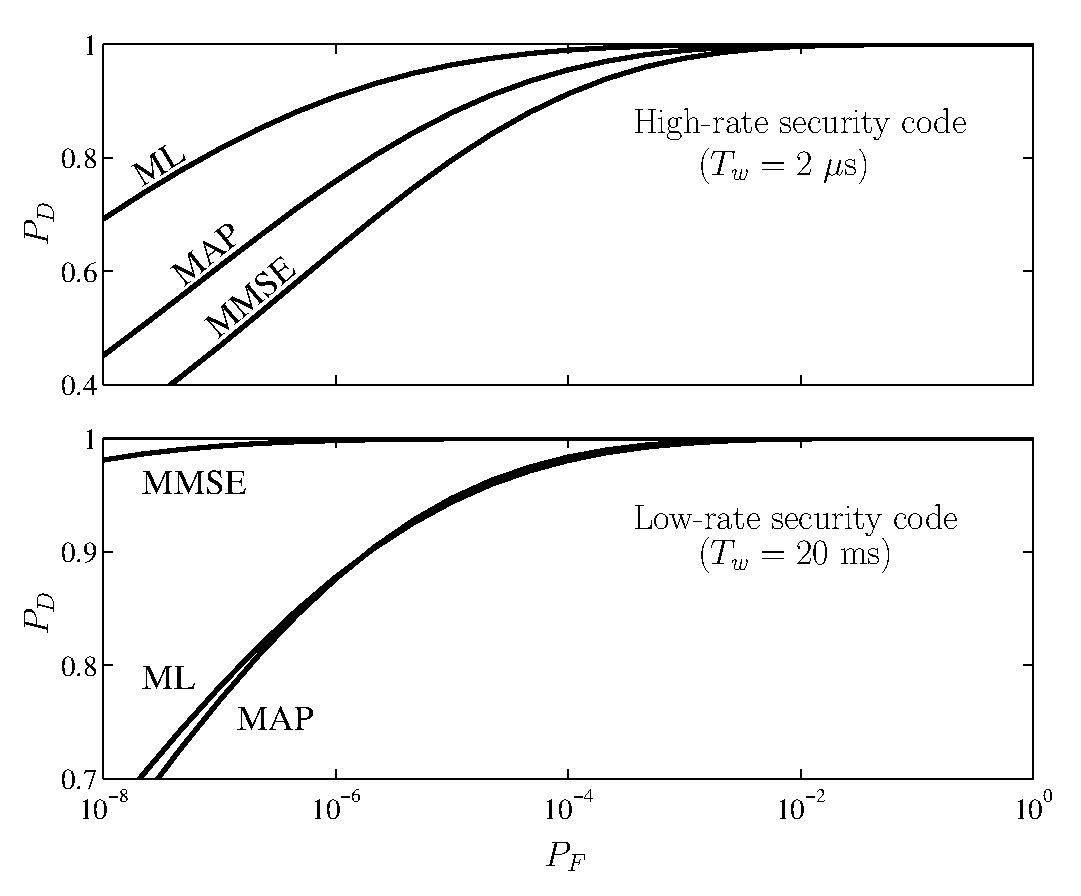
\includegraphics[width = 8.5cm]
{figs/rocplot1}
\caption{ROCs for the ML, MAP, and MMSE security code estimation strategies
  under the following scenario: $(\cnr)_s = 54$ dB-Hz,
  $(\cnr)_r = 48$ dB-Hz, $\eta = 1$, $d = 0$, $N = 400$. Top panel: High-rate
  security code with $T_w = 2~ \mu$s.  Bottom panel: Low-rate security code
  with $T_w = 20$ ms.}
\label{fig:rocplot1}
\end{figure}

Sometimes you have to take up both columns with a figure, as in
Fig. \ref{fig:rx-model}.

\begin{figure*}[t]
  \centering
  \includegraphics[width=\textwidth]{figs/correlation}
  \caption{Block diagram of the standard AGC, correlation, and accumulation
    operations in a GNSS receiver. The product of the AGC-scaled incoming
    signal $\beta(t)r(t)$ and the conjugate of the local replica
    $\ell(t,\tau)$ is accumulated over $T$ seconds to produce the discrete
    complex-valued accumulation product $\xi_k(\tau)$. For notational
    convenience, the accumulation product has been scaled by $1/T$.}
  \label{fig:rx-model}
\end{figure*}

\section{Algorithms}
Use the full word Algorithm to refer to an algorithm in your paper; e.g.,
``Algorithm~\ref{algo:correlation-search} shows the pseudocode for this
process.'' Use the following format for algorithms. Note that variables should
be written in mathematical italic font, whereas functions can be written either
in typewriter font; e.g.,
\[D_{\text m} = \texttt{toOGM} \left( \bm{p}_{\text m}^{W} - \bm{t}_k^{V},
    \delta t \right)\] or in mathematical italic font.

\begin{algorithm}
  \footnotesize
  \SetKwInOut{Input}{Input}
  \SetKwInOut{Output}{Output}
  \Input{$\bm{p}_{\text m}^W$, $\bm{p}_{{\text b, } 1:k}^B$, $\bm{t}_{1:k}^{V}$, $\phi_{1:k}^{V}$, $\sigma_t$, $\sigma_\phi$, $\delta t$, $\delta \phi$}
  \vspace{0.25em}
  \Output{$\widehat{\bm{\Theta}}$}

  \vspace{1em}

  $D_{\text m} = \texttt{toOGM} \left( \bm{p}_{\text m}^W - \bm{t}_k^{V}, \delta t \right)$

  $\tilde{D}_{\text m} = \texttt{FFT2} \left( \texttt{pad} \left( D_{\text m}, 3\sigma_t \right) \right)$

  \vspace{1em}

  $\bm{p}_{{\text b, } 1:k}^{V} = R \left( \phi_{1:k}^{V} \right) \bm{p}_{{\text b, } 1:k}^B + \bm{t}_{1:k}^{V}$

  $D_{\text b} = \texttt{toOGM} \left( \bm{p}_{{\text b, } 1:k}^{V} - \bm{t}_k^{V}, \delta t \right)$

  $\tilde{D}_{\text b} = \texttt{FFT2} \left( \texttt{pad} \left( D_{\text b}, 3\sigma_t \right) \right)$

  \vspace{1em}

  $n = 3\sigma_t / \delta t$

  $m = 3\sigma_\phi / \delta \phi$

  \For{i = -m:m}{ 
    $\Delta \phi = i \delta \phi$

    $\tilde{D}_{\text b}^{\Delta \phi} = \texttt{rotate2} \left( \tilde{D}_{\text b}, \Delta \phi \right)$

    $\mathsf{R}[i,:,:] = \texttt{IFFT2} \left( \tilde{D}_{\text m} \circ \texttt{conj} \left( \tilde{D}_{\text b}^{\Delta \phi} \right) \right) \left[ -n : n, -n : n \right]$
  }
  $\widehat{\bm{\Theta}} = \argmax \left( \mathsf{R} \right)$

  \caption{\texttt{fastGlobalAlign}}
  \label{algo:correlation-search}
\end{algorithm}


\begin{algorithm}
\SetKwInOut{Input}{Input}
\SetKwInOut{Output}{Output}
\Input{$\vbh{z} \in \mathbb{R}^m$, $L \in \mathbb{R}^{m \times m}$}
\Output{$\vbc{z} \in \mathbb{Z}^m$}
$\vbh{z}_{\text c} = \vbh{z}$

\For{i = 1:m}{ 
$\check{{z}}_{i}=\lfloor\hat{{z}}_{{\text c}i} \rceil$

$\check{{\epsilon}}_{{\text c}i}=\hat{{z}}_{{\text c}i} - \check{{z}}_{i}$


\For{j = i+1:m}{
$\hat{{z}}_{{\text c}j}=\hat{{z}}_{{\text c}j} - l_{ij}\check{{\epsilon}}_{{\text c}i} $\
}
}
\caption{${\text{IB}}( \vbh{z}, L)$}
\label{algo:second-algo}
\end{algorithm}
\noindent

\section{Stylistic Conventions}
\subsection{Mathematical Notation}
\begin{enumerate}
\item Define \emph{all} mathematical notation that you introduce unless it's
  been previously defined.  Where possible, introduce notation \emph{before}
  presenting the equation involving the notation.
\item Put units in straight font, not italics or math font; e.g., cm not $cm$.
\item Write subscripts that represent indices or are just one letter long in
  the usual mathematical italic font; e.g., ${x}_{ak}$.  Write subscripts that
  are words or abbreviated words in roman type: ${x}_{\text{max}}$.
\item Defining {\tt newcommand} macros for the paper can make it easier to
  repeatedly write complicated LaTeX math expressions; e.g., $\Fc{1}$, $\Fs$,
  $\Fsr$.
\end{enumerate}

\subsection{Punctuation}
Use American Style punctuation.
\href{https://www.thepunctuationguide.com/british-versus-american-style.html}{This}
website is a good reference. Note that American style quotations include
commas and periods within the quotation, even if they are not actually part of
what was quoted; e.g.,
\begin{quotation}
  “Economic systems,” according to Professor White, “are an inevitable
  byproduct of civilization, and are, as John Doe said, ‘with us whether we
  want them or not.’”
\end{quotation}
This style is not as sensible as British English, but it's the convention on
this side of the pond.  

\subsection{Abbreviations}
\begin{enumerate}
\item With few exceptions, define all abbreviations/acronyms used in
  the paper (e.g., UAV, GNSS, IMU, etc.).  Exceptions are those that have
  become so common that they're part of everyday vernacular (radar, GPS). 
\end{enumerate}

\subsection{References}
\begin{enumerate}
\item Never start a sentence with the actual numerical citation (e.g., ``[2]
  presents an optimal ...'').  Prefer instead ``Reference [2] ...'' or ``The
  authors of [2]...'' or ``Durge et al. present in [2] an optimal ...''
\end{enumerate}

\subsection{Signposts}
Busy readers rarely read a paper straight through from abstract to conclusions.
Instead, they tend to sample bits and pieces \emph{a la carte}.  For these
readers, and even for sequential readers who may need some guidance on where
they are and what is to come, it's helpful to start off each major section with
a \emph{signpost}---a brief summary of what the reader now knows and what he
can expect to learn from that section.  Sometimes the section title, perhaps in
combination with the first sub-section title, sufficies.  In other cases, a few
sentences are needed to orient the reader.  Here is an example of a
few-sentence signpost at the beginning of a section:
\begin{quotation}
  The model of road user behavior presented above applies to human
  decisions. Autonomous vehicles are likely to respond very differently,
  because they are fundamentally unable to win the game of chicken. Moreover,
  they are likely to obey the rules of the road far more than human drivers,
  particularly in safety-critical situations. This section elaborates such
  reasoning.
\end{quotation}


\section{Conclusions}
Like the abstract, this section should give a recap of the whole paper.  Write
in simple past tense.  Don't assume the reader has read the paper.

Example:\\

A real-time kinematic (RTK) positioning system tailored for urban vehicular
positioning has been described and evaluated.  To facilitate performance
comparison against similar systems, the system was tested without any benefit
of aiding by inertial or electro-optical sensors.  Over nearly 2 hours of
urban testing, including multiple passes through Austin's dense urban center,
the system achieved an 85\% probability of correct integer fix for a 2.4\%
probability of incorrect fix, resulting in 3D positioning errors smaller than
17 cm (95\%).  A performance sensitivity analysis revealed that navigation
data bit prediction on fully-modulated GNSS signals is key to high-performance
urban RTK positioning, and that a dense reference network, carrier tracking
bandwidth adaptation, and rover antenna calibration each offer a significant
integrity benefit. A comparison with existing unaided systems for urban GNSS
processing indicates that the proposed system has a significant advantage in
availability and/or accuracy.

\section*{Acknowledgments}
Example:\\

This work was supported in part by the U.S. Department of Transportation (USDOT)
under the University Transportation Center (UTC) Program Grant 69A3552047138
(CARMEN), and by affiliates of the 6G@UT center within the Wireless Networking
and Communications Group at The University of Texas at Austin.

\bibliographystyle{ieeetran} 
\bibliography{pangea}
\end{document}

